\documentclass[9pt, aspectratio=169]{beamer}
%\documentclass[9pt, aspectratio=169, handout]{beamer}

\usetheme{metropolis}
\setbeamertemplate{itemize items}{\faAngleRight}

\metroset{titleformat=smallcaps,block=fill,numbering=counter,progressbar=frametitle,sectionpage=none}
\setbeamersize{text margin left=5mm,text margin right=5mm} 
% \input{embed_video}
\usepackage{fontspec}
\usepackage[scale=1]{ccicons}
\usepackage{metalogo}
\usepackage{xcolor,colortbl}
\usepackage{multicol,multirow,booktabs}
\usepackage{appendixnumberbeamer}
\usepackage{graphicx}
\usepackage{svg}
\usepackage{mismath}
\usepackage{bm}
\usepackage{fontawesome5}
\usepackage{csquotes}
%\usepackage[backend=biber, natbib, sorting=nyt, doi=true, url=false, url=false, isbn=false, maxbibnames=10]{biblatex}
%\addbibresource{../../utils/refs.bib}

\usepackage[spanish, es-nodecimaldot]{babel}
\deftranslation[to=spanish]{Definition}{Definición}
\deftranslation[to=spanish]{Theorem}{Teorema}
\deftranslation[to=spanish]{Example}{Ejemplo}

\usepackage{mathtools, mathrsfs}
\usefonttheme{professionalfonts}
\usepackage{textcomp, wasysym}

\setsansfont[BoldFont={Iwona Bold}, Numbers={Lining, Proportional}]{Iwona Light}
% \setmathsfont(Digits)[Numbers={Lining, Proportional}]{Fira Sans Light}
\setmonofont[Scale=MatchLowercase]{DejaVu Sans Mono}

\setbeamercolor{alerted text}{fg=red,bg=black!2}
\setbeamercolor{progress bar}{fg=red,bg=red!2}
\setbeamertemplate{itemize item}{\faCaretRight}
\setbeamertemplate{itemize subitem}{ \faAngleRight}
\setbeamertemplate{blocks}[shadow=false]
\setbeamercolor{block title}{bg=black!30,fg=red}
\setbeamercolor{block body}{bg=black!20,fg=black}
\setbeamertemplate{theorem begin}
{%
\begin{\inserttheoremblockenv}
{%
\inserttheoremheadfont
%{Teorema:}
\inserttheoremname
\ifx\inserttheoremaddition\@empty\else\ : \inserttheoremaddition\fi%
\inserttheorempunctuation
}%
}
\setbeamertemplate{theorem end}{\end{\inserttheoremblockenv}}
\makeatother


 
\usepackage{gensymb,amssymb}
\usepackage{siunitx}
\DeclareSIUnit{\nada}{\relax}
\usepackage{upquote}
\usepackage{cancel}
\usepackage{algpseudocode}
\algrenewcommand\algorithmicrequire{\textbf{Requiere}}
\algrenewcommand\algorithmicensure{\textbf{Devuelve}}
\setbeamertemplate{blocks}[shadow=false]

\newcommand{\cx}{\column{0.5\textwidth}}
\newcommand{\cw}[1]{\column{#1\textwidth}}

\author{Manuel Carlevaro}
\date{}
\institute{
  \vspace{6em}
  \centering
  {\small
  Universidad de Navarra \enspace • \enspace 2024 
} }

%% Operadores
\DeclareMathOperator{\sen}{sen}
\DeclareMathOperator{\senc}{senc}
\DeclareMathOperator{\sign}{sign}
\newcommand{\T}[1]{\underline{\bm{#1}}}
\DeclareMathOperator{\Tr}{Tr}
\DeclareMathOperator{\rg}{rg}
\DeclareMathOperator{\cond}{cond}

\usepackage{hyperref}
\hypersetup{
    colorlinks,
    citecolor=blue,
    filecolor=black,
    linkcolor=blue,
    urlcolor=blue
}
\urlstyle{same}


\usepackage{tikz}
\usetikzlibrary{shapes,shadows,arrows,positioning,matrix,chains,backgrounds,fit}

\tikzset{
    %Define standard arrow tip
    >=stealth',
    %Define style for boxes
    obj/.style={
           rectangle,
           rounded corners,
           draw, very thick,
           text width=10em, fill=green!20,
           minimum height=2em,
           text centered, drop shadow},
    proc/.style={
	    rectangle, rounded corners,
	    draw,fill=red!50,very thick,
	    text width=8em,minimum height=2em,
	    text centered, drop shadow},
    % Define arrow style
    pil/.style={
           ->,
           thick,
           shorten <=2pt,
           shorten >=2pt,}
}

%\setbeamertemplate{bibliography item}{%
  %\ifboolexpr{ test {\ifentrytype{book}} or test {\ifentrytype{mvbook}}
    %or test {\ifentrytype{collection}} or test {\ifentrytype{mvcollection}}
    %or test {\ifentrytype{reference}} or test {\ifentrytype{mvreference}} }
    %{\setbeamertemplate{bibliography item}{\faBook}}
    %{\ifentrytype{online}
            %{\setbeamertemplate{bibliography item}{\faGlobe}}
   %{\setbeamertemplate{bibliography item}{\faFileText}}}%
  %\usebeamertemplate{bibliography item}}

%\defbibenvironment{bibliography}
  %{\list{}
     %{\settowidth{\labelwidth}{\usebeamertemplate{bibliography item}}%
      %\setlength{\leftmargin}{\labelwidth}%
      %\setlength{\labelsep}{\biblabelsep}%
      %\addtolength{\leftmargin}{\labelsep}%
      %\setlength{\itemsep}{\bibitemsep}%
      %\setlength{\parsep}{\bibparsep}}}
  %{\endlist}
  %{\item}
%\newcommand{\bcite}[1]{\citeauthor{#1}, \citetitle{#1} (\citeyear{#1})}


\title{Introducción a las matemáticas}
\subtitle{Ecuaciones e inecuaciones}


\begin{document}
\maketitle

\begin{frame}{ Objetivos }
\begin{itemize}
    \item Mejorar las destrezas en la manipulación de expresiones algebraicas.
    \item Resolver ecuaciones e inecuaciones.
\end{itemize}
\end{frame}

\section{Introducción a las ecuaciones}

\begin{frame}{Introducción a las ecuaciones}
    Una \textbf{igualdad} es un enunciado en el que se establece que dos expresiones matemáticas son iguales. Está compuesta por \textbf{dos miembros} (izquierdo y derecho) conectados por el símbolo \textbf{igual}. Algunas igualdades son verdaderas y otras no; en otros casos, la igualdad involucra una o más variables: este tipo de igualdades se llaman \textbf{ecuaciones} que podrán ser verdaderas o falsas según los valores que tomen las variables involucradas.
    \[ \begin{underbracket}{3 \, x + 4(y-1)}_{\text{miembro izquierdo}} = \overbracket{7 \x - x^2}^{\text{miembro derecho}} \end{underbracket} \]
\pause

\text{Ejemplos:}
\begin{multicols}{2}
\begin{itemize}
    \item $3 + 5 = 8$ es una igualdad verdadera.
    \item $2 + 2 = 5$ es una igualdad falsa.
    \item $4 \mul 3 + 5$ no es una igualdad.
    \item $7 x - 3 = 0$ es una ecuación con la variable $x$. Puede ser verdadera o falsa según el valor que se le asigne a la variable.
    \item $8 x - 3 y = 8$ Es una ecuación con dos variables, $x$ y $y$. Puede ser verdadera o falsa según los valores de las variables.
    \item Una \textbf{identidad} es una igualdad que vale \textbf{siempre} para cualquier valor que tomen las variables: $(a + b)^2 = a^2 + 2 a b + b^2$.
\end{itemize}
\end{multicols}
\end{frame}

\begin{frame}{Introducción a las ecuaciones}
    Los posibles valores que pueden tomar las variables en una ecuación forman el \textbf{conjunto de validez} de la ecuación. Se las suele llamar \textbf{incógnitas}, por lo que el objetivo del planteo de una ecuación es determinar el o los valores de las incógnitas que hacen que la ecuación sea verdadera.

\textbf{Ejemplos:}
\begin{columns}
\cx
    \[ 7x-3 = 0 \]
   Conjunto de validez: $\{x : x \in \mathbb{R} \}$

   Con $x = 1$ la identidad es falsa:
   \begin{align*}
       7 x - 3 &= 3 \\
       7 \cdot 1 - 3 &= 0 \\
       4 &= 0 \leftarrowtail \text{ falso}
   \end{align*}
   \pause

   \cx
   \[ \frac{3}{x} + 1 = x - 1 \]
   Conjunto de validez: $\{ x : x \in \mathbb{R} - \{ 0 \} \}$ 

   Con $x = 3$ la igualdad es verdadera:
   \begin{align*}
       \frac{3}{x} + 1 &= x - 1 \\
       \frac{3}{3} + 1 &= 3 - 1 \\
       2 &= 2 \leftarrowtail \text{ verdadero}
   \end{align*}
\end{columns}
\end{frame}

\begin{frame}{Introducción a las ecuaciones}
    \textbf{Actividad 1 -- Ecuaciones.}
    \begin{enumerate}
        \item Determine si los siguientes valores de las variables son soluciones de la ecuación planteada en cada caso:
            \begin{enumerate}[a)]
                \item $x = 1$, $x = 0$, $x = -2$ para la ecuación $x(x-3) = 2$. \medskip
                \item $y = 1$, $y = 0$, $y = -2$ para la ecuación $y^2 - 3y + 2 = 0$ \medskip
            \end{enumerate}
        \item Sin hacer ninguna cuenta en la hoja, computadora o tableta, determinar la única solución de las siguientes ecuaciones:
            \begin{enumerate}[a)]
                \item $7 = b - 2$ \medskip
                \item $12 = 3 c \medskip$
                \item $t + 6 = 2 \medskip$
                \item $4x = 2$
            \end{enumerate}
    \end{enumerate}
\end{frame}

\begin{frame}{Resolución de ecuaciones}
    Dos ecuaciones que tienen \textbf{exactamente} las mismas soluciones se dicen que son \textbf{equivalentes}. El método más utilizado para la resolución de una ecuación consiste en encontrar soluciones equivalentes que sean más sencillas de resolver.

\textbf{Propiedad 1 -- Ecuaciones equivalentes:} \medskip

\begin{columns}[t]
\cx
\textbf{Suma/resta:} 
\begin{align*}
    A &= B \txt{es equivalente a} A + C = B + C \\
    A &= B \txt{es equivalente a} A - C = B - C \\
\end{align*}

\cx
\textbf{Multiplicación/división:}
\begin{align*}
    A &= B \txt{es equivalente a} A \mul C = B \mul C \\
    A &= B \txt{es equivalente a} \frac{A}{C} = \frac{B}{C}, \; C \neq 0
\end{align*}
\end{columns}

\vspace{-1em}
\begin{alertblock}{\centering \faInfoCircle}
    \begin{multicols}{2}
    Se utiliza el símbolo $\Longleftrightarrow$ para indicar que dos ecuaciones son equivalentes. Por ejemplo: 
    \[ 2 x - 3 = 0 \Longleftrightarrow 2 x = 3 \]
    También es habitual escribir dos ecuaciones que son equivalentes una debajo de la otra, \textbf{respetando que esté alineado} el símbolo ``$=$'':
    \begin{align*}
        2 x - 3 &= 0 \\
        2 x &= 3
    \end{align*}
\end{multicols}
\end{alertblock}
\end{frame}

\begin{frame}{Resolución de ecuaciones}
    \textbf{Ejemplo:} Si tomamos la edad actual de Juan y le sumamos el doble que la edad que tenía hace 5 años obtenemos el número 56. ¿Cuál es la edad actual de Juan?
\begin{columns}
\cx
\begin{itemize}
    \item Incógnita: variable $x$
    \item Conjunto de validez: $\mathbb{N}$
\end{itemize}
\textbf{Ecuación:}
\[ x + 2(x-5) = 56 \]
Separación en términos:
\[ \overbrace{x} + \overbrace{2 (\underbrace{x} - \underbrace{5})} = \overbrace{56} \]
 \cx
 \begin{align*}
     x + 2x - 10 &= 56\\
     3x - 10 {\color{red}\, + 10} &= 56 {\color{red} \, + 10} \\
     3x &= 66 \\
     \frac{3x}{\color{red}3} &= \frac{66}{\color{red}3} \\
     x &= 22
 \end{align*}
 Conjunto solución: $\{22\}$.
\end{columns}
\end{frame}

\begin{frame}{Ecuaciones lineales}
    Las ecuaciones lineales con una variable o \textbf{ecuaciones de primer orden} son aquellas que, con operaciones de suma, resta multiplicación o división, pueden llevarse a una ecuación equivalente de la forma
    \[ {\color{red} a} \, x + \, {\color{red} b} = 0 \]
    donde $x$ es la incógnita y las letras $a$ y $b$ son números constantes. Las ecuaciones lineales pueden resolverse usando las propiedades de suma/resta y multiplicación/división de las ecuaciones equivalentes.
\pause

\textbf{Actividad 2 -- Ecuaciones lineales.}

\textbf{1.} Resolver las siguientes ecuaciones lineales (\alert{verificar la solución}):
\begin{multicols}{3}
    \begin{enumerate}[a)]
        \item $5 + 4 x = 3$
    \item $ 3 r - 9 = 18 - 6 r$
    \item $2(b-5) = b + 2(1+b)$
    \item $\dfrac{1}{2} y - 2 = \dfrac{1}{3} y$
    \item $7 - 4 v + 6 = -3 v + 29 - 5 v$
    \item $\dfrac{y}{2} + \dfrac{y}{3} = \dfrac{y}{6} + 1$
    \item $\dfrac{z}{5} = \dfrac{3}{10} z + 7$
    \item $2(1-x) = 3(1 + 2x) + 5$
    \item $\dfrac{2}{3}y + \dfrac{1}{2}(y-3) = \dfrac{y + 1}{4}$
    \item $x - \dfrac{1}{3} x - \dfrac{1}{2} x - 5 = 0$
    \item $2x - \dfrac{x}{2} + \dfrac{x + 1}{4} = 6x$
    \item $(t-4)^2 = (t+4)^2 + 32$
\end{enumerate}
\end{multicols}
\end{frame}

\begin{frame}{Ecuaciones lineales}
\textbf{Actividad 2 -- Ecuaciones lineales (continuación).}

\textbf{1.} Resolver las siguientes ecuaciones lineales. ¿Qué diferencias aparecen en la cantidad de soluciones?
\begin{multicols}{3}
    \begin{enumerate}[a)]
        \item $7x+2=-x+1$
        \item $2(x+1) + 1 = 2x + 3$
        \item $3x = 2(x+2) + x$
    \end{enumerate}
\end{multicols}

\textbf{3.} Los siguientes enunciados involucran un número desconocido, ¿cuál es ese número?
\begin{enumerate}[a)]
    \item Si multiplico un número por 3 y luego le sumo 8 obtengo 23.
    \item Si resto 7 a un número y al resultado lo multiplico por 2 entonces obtengo el mismo número.
    \item  Dentro de 20 años tendré el triple de la edad que tengo ahora.
    \item  Al aumentar la longitud de los lados de un cuadrado en \qty{1}{cm} cada uno entonces su área aumenta en \qty{2}{cm}. ¿Cuánto mide el lado original del cuadrado?
\end{enumerate}
\end{frame}

\begin{frame}{Sistemas de ecuaciones}
    Un \textbf{sistema de ecuaciones} se refiere a dos o más ecuaciones que involucran a las mismas incógnitas. Se suelen agrupar con una llave a la izquierda para indicar/recordar que se trabaja con ecuaciones de manera simultánea.

\textbf{Ejemplos:}
\begin{columns}[t]
    \cw{0.3}
\textbf{Dos} ecuaciones con \textbf{dos} incógnitas:
\[ \begin{system} x+3y = 3 \\2x + 4y = x \end{system} \]
\cw{0.3}
\textbf{Tres} ecuaciones con \textbf{dos} incógnitas:
\[ \begin{system} AB+7A = 1 \\ B^2+3A = 3 \\5A + A^2 = 1 \end{system} \]
\cw{0.3}
\textbf{Dos} ecuaciones con \textbf{tres} incógnitas:
\[ \begin{system} 3x^2 + y + z + 2 = xy \\ -x + 8 zy = y^3 \end{system} \]
\end{columns}
\pause

Solución $\mapsto$ asignar valor a \textbf{todas} las incógnitas de modo que todas las ecuaciones sean verdaderas. 
\begin{columns}[t]
    \cw{0.6}
$x=4, y=-1$ \alert{no} es solución:
\[
    \begin{system}x + 3y = 3 \\2x + 4y = x \end{system} \mapsto 
    \begin{system} 4 + 3(-1) = 3 \\ 2(4) + 4(-1) = 4 \end{system} \mapsto
        \begin{system} 1 = 3 \txt{\faTimes} \\ 4 = 4 \txt{\faCheck} \end{system}
    \]
    \cw{0.4}
$x=12, y=-3$ \alert{si} es solución:
\[
    \begin{system}x + 3y = 3 \\2x + 4y = x \end{system} \mapsto 
        \begin{system} 3 = 3 \txt{\faCheck} \\ 4 = 4 \txt{\faCheck} \end{system}
    \]
\end{columns}
\end{frame}

\begin{frame}{Sistemas de ecuaciones lineales: métodos de solución}
\begin{itemize}
    \item \textbf{Sustitución:} consiste en despejar una variable en una ecuación y reemplazar en la otra. Ejemplo:
        \[ \begin{system} x + y = 3 \\ x - y = 1 \end{system} \]
        De la primera ecuacion despejamos $x$: $x = 3 - y$, y reemplazamos en la segunda: $(3-y) - y = 1$. De aquí resulta $y = 1$, y $x = 3 - y = 2$. \pause \medskip
    \item \textbf{Eliminación:} involucra sumar múltiplos de las ecuaciones (miembro a miembro) de modo de cancelar una de las variables. Ejemplo:
        \[ \begin{system} x+y = 3 \\ x - y = 1 \end{system} \]
        Sumamos miembro a miembro ambas ecuaciones:
        \[ (x + y) + (x - y) = 3 + 1 \]
        que resulta en $2x = 4$. Entonces $x=2$ y podemos sustituir este valor en cualquiera de las ecuaciones del sistema y obtener $y = 1$.
\end{itemize}
\end{frame}

\begin{frame}{Sistemas de ecuaciones lineales}
\textbf{Actividad 3 -- Sistemas de ecuaciones lineales.}

\textbf{1.} Resolver los siguientes sistemas de ecuaciones lineales.
\begin{multicols}{3}
    \begin{enumerate}[a)]
        \item \[ \begin{system} 2x + 3y = 1 \\ x + 2y = -1 \end{system} \]
        \item \[ \begin{system} z + 2 r = 1 \\ 2z + 4 = 3(z + r) \end{system} \]
        \item \[ \begin{system} 3 m + n = 3 t \\ t + n = m \\ 4 t = n + 4 \end{system} \]
    \end{enumerate}
\end{multicols}

\textbf{2.} Los siguientes enunciados involucran números desconocidos. ¿Cuáles son esos números?
\begin{enumerate}[a)]
    \item Juan tiene cinco años más que su hermana y juntos suman cuarenta y siete años.
    \item La suma de dos números es 13 y su diferencia es 5.
    \item En una canasta hay peras, manzanas y bananas; son un total de 37 frutas. Hay 7 manzanas mas que bananas y el doble de peras que manzanas.
    \item  En un bar, tres cafés y tres muffins cuestan € 16.5. Con un descuento del 10\% en el café y del 15\% en los muffins, una compra de 5 cafés y 10 muffins cuesta € 37.75. ¿Cuál es el precio de un café y de un muffin?
\end{enumerate}
\end{frame}

\begin{frame}{Ecuaciones cuadráticas}
    Las \textbf{ecuaciones cuadráticas} son ecuaciones de \textbf{de segundo grado} de la forma:
    \[ {\color{red}a} \, x^2 + {\color{red}b} \, x + {\color{red}c} = 0 \]
    donde $x$ es la incógnita y $a$, $b$ y $c$ son números fijos constantes, y $a$ es diferente de cero.
\bigskip

\textbf{Ejemplos:}
\begin{itemize}
    \item $x^2-3x-4=0$ es una ecuación cuadrática con $a = 1$, $b = -3$ y $c = -4$.
    \item $x^2 - 2 = 0$ es una ecuación cuadrática con $a = 1$, $b = 0$ y $c = -2$.
    \item $2x+3 = 0$ no es una ecuación cuadrática.
    \item $\dfrac{x^2}{3} + x = 0$ es una ecuación cuadrática con $a = 1/3$, $b = 1$ y $c = 0$.
\end{itemize}
\end{frame}

\begin{frame}{Ecuaciones cuadráticas: solución}
    \textbf{Ejemplos de casos particulares:}
\begin{multicols}{2}
\begin{itemize}
    \item Ecuación cuadrática con una única solución: $x^2 = 0$. Solución: $\{0\}$
    \item Ecuación cuadrática con dos soluciones: $x^2 = 9$. Solución: $\{-3, 3\}$
    \item Ecuación cuadrática sin soluciones: $x^2 = -4$. Solución: $\{ \varnothing \}$
    \item Ecuación cuadrática $(x+2)^2 = 9$. Solución: $\{-5, 1\}$.
\end{itemize}
\end{multicols}
\pause
\begin{columns}
\cw{0.6}
\textbf{Solución general:} fórmula de Bhaskara:
\[ x_1, x_2 = \frac{-b \pm \sqrt{b^2 - 4\, a \, c}}{2a} \]
Discriminante: $\Delta = b^2 - 4 a c$. Tres casos:
\begin{itemize}
    \item $\Delta > 0$: \textbf{dos soluciones} distintas que son $x_1 = (-b + \sqrt{\Delta})/2a$ y $x_2 = (-b - \sqrt{\Delta})/2a$.
    \item $\Delta = 0$: \textbf{solución única} que será $x_1 = -b/2a$.
    \item $\Delta < 0$: \textbf{no hay solución}.
\end{itemize}
\cw{0.3}
\begin{center}
    
\includegraphics[width=0.75\textwidth]{figs/fig-01.png}
    
    {\tiny Fuente: Wikimedia.}
\end{center}
\end{columns}
\end{frame}

\begin{frame}{Ecuaciones cuadráticas: solución}
\begin{columns}
\cw{0.60}
    \textbf{Ejemplo:} La ecuación cuadrática $x^2 + 3x + 1 = x + 9$ es equivalente a la ecuación
    \[ x^2 + 2x -8 = 0 \]
De modo que los coeficientes son $a = 1$, $b = 2$ y $c = -8$. El discriminante vale:
\[ \Delta = b^2 - 4 a c = 2^2 - 4 \cdot 1 \cdot (-8) = 36 \]
Como el $\Delta > 0$, habrá \textbf{dos soluciones} diferentes que serán:
\begin{columns}[t]
    \cx
    \begin{align*}
        x_1 &= \frac{-2 + \sqrt{2^2 - 4 \cdot 1 \cdot (-8)}}{2 \cdot 1} \\
        x_1 &= \frac{-2 + \sqrt{36}}{2} = \frac{-2+6}{2} = 2
    \end{align*}
    \cx
    \begin{align*}
        x_2 &= \frac{-2 - \sqrt{2^2 - 4 \cdot 1 \cdot (-8)}}{2 \cdot 1} \\
        x_2 &= \frac{-2 - \sqrt{36}}{2} = \frac{-2-6}{2} = -4
    \end{align*}
\end{columns} \medskip
\centering El conjunto solución es $\{-4, 2\}$.
\pause

\cw{0.35}
Las expresiones cuadráticas se pueden \textbf{factorizar}:
\[ ax^2 + bx + c = a(x - x_1)(x-x_2) \]
siempre y cuando $\Delta \geq 0$.

Del ejemplo anterior:
\[x^2 + 2x -8 = (x-2)(x+4) \]
\pause

\begin{alertblock}{\centering \faInfoCircle}
    Una ecuación puede escribirse como $f(x) = 0$ donde $f$ es una \textbf{función}. A las soluciones de la ecuación se las denomina \textbf{raíces} o \textbf{ceros} de la función $f$.
\end{alertblock}
\end{columns}
\end{frame}

\begin{frame}{Ecuaciones cuadráticas}
    \textbf{Actividad 4 -- Ecuaciones cuadráticas.} \medskip

\textbf{1.} Reescriba estos ejemplos en la forma general de una ecuación cuadrática. Indique cuáles son los coeficientes.
\begin{multicols}{3}
\begin{enumerate}[a)]
    \item $x^2 - 3x - 4 = 0$
    \item $3y^2=-27$
    \item $x^2 = 2$
    \item $3z^2+9(z+3)=9z$
    \item $x^2-1=x-2x^2$
    \item $-\dfrac{x^2}{4} + \dfrac{2}{3} x^ 2 = 3x-1$
\end{enumerate}
\end{multicols}

\textbf{2.} Determine el conjunto de soluciones de las siguientes ecuaciones cuadráticas.
\begin{multicols}{3}
    \begin{enumerate}[a)]
        \item $x^2 - 81 = 0$ 
        \item $9(y+1)^2 = 4$
        \item $a^2 + 2 = 6a$
        \item $2x^2+4=0$
        \item $x(x-3)+2=0$
        \item $-2x^2 - \dfrac{x}{7} + 1 = 0$
    \end{enumerate}
\end{multicols}

\textbf{3.} Encuentre los valores de $k$ para que las siguientes ecuaciones tengan una única solución.
\begin{multicols}{2}
    \begin{enumerate}[a)]
        \item $x^2 - 2 k x + 4=0$
        \item $x^2 + 2 k x = 3$
    \end{enumerate}
\end{multicols}
\end{frame}

\begin{frame}{Ecuaciones cuadráticas}
    \textbf{Actividad 4 -- Ecuaciones cuadráticas (continuación).} \medskip

\textbf{4.} Factorice las siguientes expresiones cuadráticas:
\begin{multicols}{3}
\begin{enumerate}[a)]
    \item $x^2 - 81$
    \item $9(y+1)^2-4$
    \item $x(x-3)+2$
    \item $2x^2+4$
    \item $x^2 - 6x +2$
\end{enumerate}
\end{multicols}

\textbf{5.} Resuelva los siguientes problemas
\begin{enumerate}[a)]
    \item Se realiza una reunión y todas las personas se saludan entre sí con un apretón de manos; en total se producen 66 apretones. ¿Cuántas personas hay en la reunión?
    \item Mi edad actual multiplicada por mi edad hace 6 años da como resultado 216. ¿Cuál es mi edad?
    \item Al aumentar la longitud de las aristas de un cubo en \qty{1}{cm} cada una, su volumen aumenta en \qty{7}{cm^3}. ¿Cuánto mide la arista original del cubo?
\item Los lados de un rectángulo miden \qty{2}{cm} y \qty{3}{cm}. Si cada uno de ellos aumenta una cantidad $x$ de centímetros entonces el área aumenta al doble. ¿Cuánto vale $x$?
\end{enumerate}
\end{frame}

\begin{frame}{Sistemas mixtos}
    Los sistemas mixtos pueden estar conformados por ecuaciones de cualquier tipo: aquí trabajaremos con sistemas que incluyen \textbf{ecuaciones lineales} y \textbf{ecuaciones cuadráticas}.

\textbf{Ejemplo:}
\begin{columns}
\cx
\[ \begin{system} -x^2 + 2 x + y =- 3 \\ 2x + y = 1 \end{system} \]

Solución por sustitución: Despejamos $y$ de la segunda ecuación:
\[ y = 1 - 2x \]
y sustituimos en la primera:
\begin{align*}
-x^2 +2x +(1-2x) &= -3 \\
x^2 - 2x - (1-2x) - 3 &= 0 \\
x^2 - 2x - 1 + 2x -3 &= 0 \\
x^2 - 4 &= 0 \\
(x-2)(x+2) &= 0
\end{align*}
Solución para $x$: $\{-2, 2\}$.
\cx
Reemplazando cada solución de $x$ en la ecuación para $y$:

\[ x_1 = -2 \mapsto y_1 = 1 - 2 x_1 = 1 - 2(-2) = 5 \]
\[ x_2 = 2 \mapsto y_1 = 1 - 2 x_2 = 1 - 2(2) = -3 \]

\begin{center}
    \includegraphics[width=0.7\textwidth]{figs/mixtos.pdf}
\end{center}
\end{columns}
\end{frame}

\begin{frame}{Sistemas mixtos}
    \textbf{Actividad 5 -- Sistemas de ecuaciones mixtos.}

\textbf{1.} Resuelva los siguientes sistemas de ecuaciones mixtos. 
\begin{multicols}{4}
    \begin{enumerate}[a)]
        \item \[ \begin{system} x^2 + y^2 = 5 \\ x + y = 3 \end{system} \] 
        \item \[ \begin{system} x^2 + 3y^2 = 4 \\ y - x^2 = 0 \end{system} \]
        \item \[ \begin{system} xy + 9 = 0 \\ 6 + y = x \end{system} \]
        \item  \[ \begin{system} x^2 + y^2 + z^2 = 1 \\ x + y + z = 1 \\ x + y = 1 \end{system} \]
    \end{enumerate}
\end{multicols}

\textbf{2.} Resuelva los siguientes problemas. 
    \begin{enumerate}[a)]
\item ¿Existe algún rectángulo cuya área sea \qty{12}{m^2} y su perímetro sea \qty{8}{m} ?
        \item Los lados de un rectangulo miden \qty{7}{m} y \qty{12}{m}, ¿En cuánto se debe aumentar el ancho y en cuánto se debe disminuir el largo para que el perímetro aumente en \qty{2}{m} y el área permanezca igual?
        \item La suma de las áreas de dos cuadrados da \qty{5}{cm^2} y la suma de sus perímetros da \qty{12}{cm}. ¿Cuánto valen las longitudes de los lados de cada cuadrado?
    \end{enumerate}
\end{frame}

\section{Desigualdades e inecuaciones}
\begin{frame}{Desigualdades e inecuaciones}
    \begin{definition}[Desigualdad]
        Una \textbf{desigualdad} es un enunciado que establece que una expresión numérica es más grande que otra. Al igual que las igualdades, están compuestas por dos miembros conectados con alguno de los cuatro símbolos siguientes:
        \begin{multicols}{2}
            \begin{itemize}
                \item $<$ : \textbf{menor que}.
                \item $>$ : \textbf{mayor que}.
                \item $\leq$ : \textbf{menor o igual que}.
                \item $\geq$ : \textbf{mayor o igual que}.
            \end{itemize}
        \end{multicols}
    \end{definition}
\pause

\textbf{Ejemplos:}
\begin{columns}
\cw{0.75}
\begin{multicols}{2}
\begin{itemize}
\item $4 < 8$ : verdadero
\item $8 > 4$ : verdadero
\item $5 > 9$ : falso
\item $7 \leq 7$ : verdadero
\item $2 \leq 7 $ : verdadero
\item $2 x + 1 \geq 3$ : inecuación con una variable
\item $2 > 2$ : desigualdad falsa
\item $2 \geq 2$ : desigualdad verdadera
\item $-5 > -9$ : verdadera
\end{itemize}
\end{multicols}
\end{columns}
\end{frame}

\begin{frame}{Desigualdades e inecuaciones}
Las inecuaciones son desigualdades donde aparecen una o más incógnitas y pueden resolverse planteando inecuaciones equivalente que sean más sensillas. Se utilizan las siguientes propiedades:

\textbf{Propiedad 2 -- Desigualdades y operaciones}

\textbf{Suma/resta:} Al sumar o restar el mismo número a ambos miembros de una desigualdad, se \textbf{mantiene} la desigualdad. Simbólicamente:
\begin{columns}
    \cx
    \[ A < B \text{ es equivalente a } A \mathcolor{red}{+C} < B  \mathcolor{red}{+C} \]
    \cx
    \[ A < B \text{ es equivalente a } A \mathcolor{red}{-C} < B  \mathcolor{red}{+C} \]
\end{columns} \medskip

\textbf{Multiplicación/división:} \medskip

\begin{columns}
\cw{.45}
\textbf{Caso $C>0$:} al multiplicar o dividir ambos miembros de una desigualdad por un número \textbf{positivo}, se \textbf{mantiene} la desigualdad:
\[ A < B \text{ es equivalente a } A \mathcolor{red}{\mul C} < B \mathcolor{red}{\mul C} \] 
\[ A < B \text{ es equivalente a } \frac{A} {\mathcolor{red}{C}} < \frac{B}{\mathcolor{red}{C}} \] 
\cw{.45}
\textbf{Caso $C<0$:} al multiplicar o dividir ambos miembros de una desigualdad por un número \textbf{negativo}, se \textbf{invierte} la desigualdad:
\[ A < B \text{ es equivalente a } A \mathcolor{red}{\mul C} > B \mathcolor{red}{\mul C} \] 
\[ A < B \text{ es equivalente a } \frac{A}{\mathcolor{red}{C}} > \frac{B}{\mathcolor{red}{C}} \] 
\end{columns}
\end{frame}

\begin{frame}{Desigualdades e inecuaciones}
    \textbf{Actividad 6 -- Desigualdades e inecuaciones.}
{\small

\textbf{1.} Indique para cada caso qué signo, $>$, $<$, $\leq$ o $\geq$ correspondientes en los espacios para que la desigualdad sea verdadera:
\begin{multicols}{4}
\begin{enumerate}[a)]
    \item $3 \; \underline{\hspace{0.5cm}} \; \dfrac{7}{2}$
    \item $-3 \; \underline{\hspace{0.5cm}} \; -\dfrac{7}{2}$
    \item $3.5 \; \underline{\hspace{0.5cm}} \; \dfrac{7}{2}$
    \item $\dfrac{2}{3} \; \underline{\hspace{0.5cm}} \; 0.67$
    \item $\dfrac{2}{3} \; \underline{\hspace{0.5cm}} \; -0.67$
    \item $-4 \; \underline{\hspace{0.5cm}} \; -3$
    \item $-33 \; \underline{\hspace{0.5cm}} \; -4$
\end{enumerate}
\end{multicols}

\textbf{2.} Indique cuáles de las siguientes desigualdades son verdaderas y cuáles falsas.
\begin{multicols}{4}
    \begin{enumerate}[a)]
        \item $-6 < -10$
        \item $-\dfrac{1}{2} < -1$
        \item $-2 \leq -2$
        \item $10^4 > 31452$
    \end{enumerate}
\end{multicols}

\textbf{3.} Las expresiones de la Propiedad 2 -- Desigualdades y operaciones (suma/resta y multiplicación/división) fueron presentadas con el símbolo $<$. Escriba los mismos enunciados con los símbolos $<$, $\leq$ y $\geq$.

\textbf{4.} Escriba los siguientes enunciados con símbolos de desigualdades:
\begin{multicols}{3}
    \begin{enumerate}[a)]
        \item $x$ es positiva
        \item $b$ es menor a 4
        \item $t$ es mayor o igual a $-2$
        \item $y$ es negativa
        \item $y$ no es negativa
        \item $a$ no es mayor a 0
    \end{enumerate}
\end{multicols}
}
\end{frame}

\begin{frame}{Desigualdades e inecuaciones}
\textbf{Intervalos numéricos:}
{\small
\begin{columns}
\cw{0.5}
\begin{definition}[Intervalo abierto]
Para dos números con $a < b$ se llama \textbf{intervalo abierto} a todos los números que están entre $a$ y $b$ \textbf{sin incluirlos} y lo escribimos $(a, b)$
\[ (a, b) = \{x : a < x < b \} \]
\begin{center}
    
\includegraphics[width=0.7\textwidth]{figs/fig-02.pdf}
\end{center}
\end{definition}
\cw{0.5}
\begin{definition}[Intervalo cerrado]
    Se llama \textbf{intervalo cerrado} a los números que están entre $a$ y $b$ \textbf{inlcuyendo a los bordes} y lo escribimos $[a, b]$
    \[ [a, b] = \{x : a \leq x \leq b \} \]
\begin{center}
    
\includegraphics[width=0.7\textwidth]{figs/fig-03.pdf}
\end{center}
\end{definition}
\end{columns}
\pause

\begin{alertblock}{\centering \faInfoCircle}
    Se utilizan \textbf{corchetes} $[\,]$ para los casos de intervalos cerrados, y \textbf{paréntesis} $(\,)$ para los casos de intervalos abiertos o cuando el conjunto no tiene fin en alguna dirección, que indicamos con los símbolos $\infty$ o $-\infty$ que se leen \textbf{infinito} o \textbf{menos infinito}. 
\begin{columns}
\cw{0.4}
\begin{align*} \{x : 3 < x \} &= \{x : x \txt{es un número mayor que} 3 \} \\
&= (3, \infty) \end{align*}
\begin{center}
    
\includegraphics[width=0.5\textwidth]{figs/fig-04.pdf}
\end{center}
\cw{0.4}
Los símbolos $\infty$ y $-\infty$ \textbf{no son números}. Son solo símbolos que se utilizan para indicar que el intervalo comienza en un cierto número $a$ y no tienen final hacia la derecha o hacia la izquierda.
\end{columns}
\end{alertblock}
}
\end{frame}

\begin{frame}{Desigualdades e inecuaciones}
    \textbf{Ejemplos:} \medskip

    \textbf{1.} El conjunto de los números reales comprendidos entre -1 y 4:
\[ \{x : -1 < x < 4 \} = (-1, 4) \]
\begin{center}
    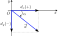
\includegraphics[width=0.3\textwidth]{figs/fig-05.pdf}
\end{center}

\textbf{2.} El conjunto de los números reales menores o iguales que $2$:
\[ \{x : x \leq 2 \} = (-\infty, 2] \]
\begin{center}
    
\includegraphics[width=0.3\textwidth]{figs/fig-06.pdf}
\end{center}
\end{frame}

\begin{frame}{Desigualdades e inecuaciones}
\textbf{Actividad 7 -- Intervalos numéricos.}

\textbf{1.} Completar la siguiente tabla:
\begin{center}
\begin{tabular}{rccc}
\toprule
     & \textbf{Conjunto} & \textbf{Intervalo} & \textbf{Representación gráfica} \\
\midrule
     Intervalo abierto & $\{x : a < x < b\}$ & $(a, b)$ & 
\includegraphics[width=0.2\textwidth]{figs/fig-02.pdf} \\
     \midrule
     Intervalo cerrado & & $[a, b]$ \\
     \midrule
     Intervalo semi-abierto & $\{x : a < x \leq b\}$ & & 
\includegraphics[width=0.2\textwidth]{figs/fig-07.pdf} \\
     \midrule
     Intervalo semi-abierto & $\{x : a \leq x <b\}$ & & \\
     \midrule
     Semirecta cerrada & $\{ x : a \leq x \}$ & $[a, \infty)$ & \\
     \midrule
     Semirecta abierta & & $(-\infty, b)$ & 
\includegraphics[width=0.2\textwidth]{figs/fig-08.pdf} \\
     \midrule
     Semirrecta abierta & $\{x : a < x \}$ & & \\
     \midrule
     Semirrecta cerrada & & $(-\infty, b]$ & \\
     \bottomrule
\end{tabular}  
\end{center}
\end{frame}


\begin{frame}{Desigualdades e inecuaciones}
\textbf{Actividad 7 -- Intervalos numéricos (continuación).}
\medskip

\begin{columns}[t]
\cw{0.45}
\textbf{2.} Escriba en forma de intervalo y en forma de conjunto los siguientes intervalos: \\[1em]
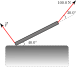
\includegraphics[scale=0.7]{figs/fig-09.pdf}

\textbf{3.} Dibuje en una recta real los siguientes intervalos:
\begin{multicols}{3}
    \begin{enumerate}[a)]
        \item $\left[ \dfrac{1}{2}, 5 \right)$
        \item $(-\infty, 0)$
        \item $(0,1)$
        \item $\left(-3, \dfrac{1}{2} \right] $
        \item $[25 ,\infty)$
    \end{enumerate}     
\end{multicols}
\cw{0.5}
\textbf{4.} Realice las siguientes operaciones entre intervalos. Las respuestas deben estar en forma de intervalo.
\begin{multicols}{2}
    \begin{enumerate}[a)]
        \item $(-2, 5) \cup (4, 6]$
        \item $(-2, 5/3) \cap (1, 6]$
\item $(-\infty, 0] \cup (-2, 3)$
\item $[1, 4) \cup [4, 8)$
\item $[0,3] - (2, 4)$
\item $[0, 3] - (4, 5)$
\item $\mathbb{R} - (2, +\infty)$
\item $(-\infty, 3) - \{0\}$
\item $(-2/3, 4/3) \cup \{5/4\}$
    \end{enumerate}
\end{multicols}
\end{columns}
\end{frame}

\begin{frame}{Desigualdades e inecuaciones}
\textbf{Resolución de inecuaciones lineales:} se usa el mismo método que para la resolución de ecuaciones lineales, pasando por sucesivas inecuaciones equivalentes. Hay que tener en cuenta las propiedades de las desigualdades de la suma/resta y multiplicación/división.

\textbf{Ejemplo:} Una fábrica A le paga a sus vendedores € 100 por artículo más una cantidad fija de € 3.000. La competencia B le paga a sus vendedores € 150 por artículo más una cantidad fija de € 3.000. ¿Cuántos artículos tienen que vender los de la competencia B para ganar más que el de la fábrica A?
\begin{columns}
\cw{0.6}
\begin{itemize}
    \item Ganancia vendedor A: $100 x + 5000$
    \item Ganancia vendedor B: $150 x + 3000$
\end{itemize}
Resolver:
\[ 100 x + 5000 < 150 x + 3000 \]
\begin{align*}
100 &x + 5000 \mathcolor{red}{-5000} < 150 x + 3000 \mathcolor{red}{ -5000 } \Longleftrightarrow 100 x < 150 x - 2000 \\
100 &x - 150 x < 150x - 2000 - 150x \Longleftrightarrow -50 x < -2000
\end{align*}
\cw{0.4}
(Multiplicar por un número negativo invierte la desigualdad)
\[ \frac{-50 x}{-50} > \frac{-2000}{-50} \Longleftrightarrow x > 40 \]
\end{columns}
\end{frame}

\begin{frame}{Ecuaciones e inecuaciones}
    \textbf{Actividad 8 -- Resolución de desigualdades.}

    \textbf{1.} Resolver las siguientes inecuaciones. Escriba los conjuntos solución con la notación de intervalos.
\begin{multicols}{3}
\begin{enumerate}[a)]
    \item $5 + 4 x > 17$
    \item $-1 -a \leq 2 a - 3$
    \item $2 y > 2(y-1)$
    \item $-B \geq -(B-5)$
    \item $\dfrac{x}{2} + 3 < 2 x - 6 $
    \item $\dfrac{2 + 3x}{3} \geq x + \dfrac{x + 1}{2} $
\end{enumerate}
\end{multicols}

\textbf{2.} Resuelva la siguiente situación.
\begin{quote}
    En un sistema de reparto a domicilio sólo se aceptan paquetes en forma de caja de zapatos que cumplan que el largo más dos veces el ancho más dos veces el alto no sea mayor a \qty{275}{cm}.
\end{quote} 
\vspace{-2em}
\begin{enumerate}[a)]
\item ¿Se aceptará un paquete con \qty{15}{cm} de ancho, \qty{20}{cm} de alto y \qty{13}{cm} de largo?
\item ¿Cuánto puede medir el alto de un paquete aceptable que tiene una base cuadrada de \qty{23}{cm} de cada lado?
\item ¿Cuánto puede medir el ancho de un paquete aceptable que tiene \qty{10}{cm} de alto y \qty{20}{cm} de largo?
\end{enumerate}
\end{frame}

\begin{frame}{Desigualdades e inecuaciones} 
    \textbf{Resolución de sistemas de inecuaciones lineales.} {\small Para encontrar el conjunto solución de un sistema de inecuaciones lineales, en primer lugar se resuelve cada inecuación, es decir, encontramos el conjunto solución de cada una de las inecuaciones del sistema. Luego, para que el sistema tenga solución, todas las inecuaciones tienen que satisfacerse simultáneamente, por lo que hay que encontrar los números que cumplen todas las condiciones a la vez. }

\begin{columns}[t]
{\small 
\cw{0.45} 
\textbf{Ejemplo:} Resolver
\[ \begin{system} 4x + 3 > x + 9 \\ -2x + 6 > -15 + 5 x \end{system} \]
\begin{align*}
    4x + 3 > x + 9 &\Longleftrightarrow 4x - x > 9 - 3 \\
                   &\Longleftrightarrow 3 x > 6 \\
                   &\Longleftrightarrow x > 2
\end{align*}
Solución: $P = (2, +\infty)$
\begin{center}
    
\includegraphics[width=0.7\textwidth]{figs/fig-10.pdf}
\end{center}

\cw{0.55}
\begin{align*}
    -2x + 6 > -15 + 5 x &\Longleftrightarrow -2x -5x > -15 -6 \\
                        &\Longleftrightarrow -7x > -21 \\
                        &\Longleftrightarrow x < \frac{-21}{-7} \\
                        &\Longleftrightarrow x < 3
\end{align*}
Solución: $S = (-\infty, 3)$
\begin{center}
    
\includegraphics[width=0.7\textwidth]{figs/fig-11.pdf}
\end{center}
Solución del sistema: $P \cap S = (2, 3)$
\begin{center}
    
\includegraphics[width=0.7\textwidth]{figs/fig-12.pdf}
\end{center}
}
\end{columns}
\end{frame}

\begin{frame}{Desigualdades e inecuaciones}
\textbf{Actividad 9 -- Resolución de sistemas de inecuaciones}

\textbf{1.} Encuentre los valores de $x$ que cumplen cada par de desigualdades en forma simultánea. También escriba las soluciones con la notación de intervalo.

\begin{multicols}{3}
    \begin{enumerate}[a)]
        \item \[ \begin{system} x+3>0 \\ x+1 < 1 \end{system} \]
        \item \[ \begin{system} x-1 \geq 3 \\ 2 < 2x + 1 \end{system} \]
        \item \[ \begin{system} \dfrac{3}{4} x + 1 \leq 2 \\ 4 - 3x \leq 0 \end{system} \]
    \end{enumerate}
\end{multicols}

\end{frame}


\end{document}
